\documentclass[paper=A4, oneside, final, DIV=30, footheight=1pt]{scrartcl} % DIV parameter deals with the division factor for box construction http://tex.stackexchange.com/a/4383
% \usepackage[top=1cm, bottom=1.2cm, left=1cm, right=1cm % http://tex.stackexchange.com/a/248127
%     showframe <- only to show the page layout
% ]{geometry}

\usepackage[portuguese, english]{babel}
\usepackage[latin1]{inputenc}
\usepackage[T1]{fontenc}
\usepackage{soul}
\usepackage{scrpage2}
\usepackage{titlesec}
\usepackage{marvosym}
\usepackage{tabularx,colortbl}
\usepackage{ifthen}
\usepackage{setspace}
\usepackage[bookmarks=false]{hyperref}

\usepackage{csquotes}
\MakeOuterQuote{"}

\hypersetup{
	unicode=false,          % non-Latin characters in Acrobat's bookmarks
	pdftoolbar=false,       % show Acrobat's toolbar?
	pdfmenubar=false,       % show Acrobat's menu?
	pdffitwindow=false,     % window fit to page when opened
	pdfstartview={FitH},    % fits the width of the page to the window
	pdftitle={Curriculum Vitae},    					% title
	pdfauthor={Eduardo Mucelli Rezende Oliveira},     % author
	pdfsubject={Curriculum Vitae},   % subject of the document
	pdfcreator={LaTeX},     % creator of the document
	pdfproducer={Rubber},   % producer of the document
	pdfnewwindow=true,      % links in new window
	colorlinks=true,        % false: boxed links; true: colored links
	linkcolor=blue,         % color of internal links
	citecolor=green,        % color of links to bibliography
	filecolor=magenta,      % color of file links
	urlcolor=blue           % color of external links
}

\urlstyle{same}                                                              % font da URL fica igual a do resto do curriculo
\titleformat{\section}{\large\scshape\raggedright}{}{0em}{}[\titlerule]
\pagestyle{scrheadings}
\renewcommand{\headfont}{\normalfont\rmfamily\scshape}
\newcommand{\gray}{\rowcolor[gray]{.90}}                                     % defini��o de um novo comando, 'gray' que seta a linha com 90% de cinza
\newcommand{\graycell}{\cellcolor[gray]{0.90}}

% ==================
% Boolean flags

\newboolean{en}
\setboolean{en}{true}           % true gera curriculo em ingles
\newboolean{pt}
\setboolean{pt}{false}          % true gera curriculo em portugues

\newboolean{academy}            % this curriculum focus a company, or academy?
\setboolean{academy}{true}

\newboolean{everything}
\setboolean{everything}{false}  % false gera curriculo so com as coisas mais recentes

% ==================

\newcommand{\course}{\ifthenelse{\boolean{en}}      {Course}{Curso}}
\newcommand{\type}{\ifthenelse{\boolean{en}}        {Type}{Tipo}}
\newcommand{\period}{\ifthenelse{\boolean{en}}      {Period}{Per�odo}}
\newcommand{\institution}{\ifthenelse{\boolean{en}} {Institution}{Institui��o}}
\newcommand{\avgscore}{\ifthenelse{\boolean{en}}    {Avg.Score}{Nota M�dia}}
\newcommand{\score}{\ifthenelse{\boolean{en}}       {Score}{Nota}}
\newcommand{\area}{\ifthenelse{\boolean{en}}        {Area}{�rea}}
\newcommand{\project}{\ifthenelse{\boolean{en}}     {Project}{Projeto}}
\newcommand{\pdescription}{\ifthenelse{\boolean{en}}{Description}{Descri��o}}

\newcommand{\ufmg}{\ifthenelse{\boolean{en}}        {Federal University of Minas Gerais}{Universidade Federal de Minas Gerais}}
\newcommand{\puc}{\ifthenelse{\boolean{en}}         {Pontifical Catholic University of Minas Gerais}{Pontif�cia Universidade Cat�lica de Minas Gerais}}
\newcommand{\ecole}{\ifthenelse{\boolean{en}}       {�cole Polytechnique}{�cole Polytechnique}}

\newcommand{\ufmglinked}{\ifthenelse{\boolean{en}}  {\href{http://www.ufmg.br}{Federal University of Minas Gerais}}
																			  {Universidade Federal de Minas Gerais}}
\newcommand{\puclinked}{\ifthenelse{\boolean{en}}   {\href{http://www.pucminas.br}{Pontifical Catholic University of Minas Gerais}}
																				  {Pontif�cia Universidade Cat�lica de Minas Gerais}}
\newcommand{\ecolelinked}{\ifthenelse{\boolean{en}} {\href{http://www.polytechnique.edu}{�cole Polytechnique}}
													{\href{http://www.polytechnique.edu}{�cole Polytechnique}}}

\newcommand{\france}{\ifthenelse{\boolean{en}}      {France}{Fran�a}}
\newcommand{\brazil}{\ifthenelse{\boolean{en}}      {Brazil}{Brasil}}

\newcommand{\january}{\ifthenelse{\boolean{en}}     {January }{Janeiro }}
\newcommand{\february}{\ifthenelse{\boolean{en}}    {February }{Fevereiro }}
\newcommand{\march}{\ifthenelse{\boolean{en}}       {March }{Mar�o }}
\newcommand{\april}{\ifthenelse{\boolean{en}}       {April }{Abril }}
\newcommand{\may}{\ifthenelse{\boolean{en}}         {May }{Maio }}
\newcommand{\june}{\ifthenelse{\boolean{en}}        {June }{Junho }}
\newcommand{\july}{\ifthenelse{\boolean{en}}        {July }{Julho }}
\newcommand{\august}{\ifthenelse{\boolean{en}}      {August }{Agosto }}
\newcommand{\september}{\ifthenelse{\boolean{en}}   {September }{Setembro }}
\newcommand{\october}{\ifthenelse{\boolean{en}}     {October }{Outubro }}
\newcommand{\november}{\ifthenelse{\boolean{en}}    {November }{Novembro }}
\newcommand{\december}{\ifthenelse{\boolean{en}}    {December }{Dezembro }}
\newcommand{\cc}{\ifthenelse{\boolean{en}}          {Computer Science }{Ci�ncia da Computa��o }}
\newcommand{\bachelor}{\ifthenelse{\boolean{en}}    {Bachelor's degree}{Bacharelado}}
\newcommand{\master}{\ifthenelse{\boolean{en}}      {Master's degree}{Mestrado}}
\newcommand{\phd}{\ifthenelse{\boolean{en}}			{Ph.D.}{Doutorado}}
\newcommand{\wsn}{\ifthenelse{\boolean{en}}         {Wireless Sensor Networks}{Redes de Sensores sem Fio}}
\newcommand{\complex}{\ifthenelse{\boolean{en}}     {Complex Networks}{Redes Complexas}}
\newcommand{\data}{\ifthenelse{\boolean{en}}     	{Large-scale Data Analysis}{An�lisa de Dados em Larga Escala}}
\newcommand{\research}{\ifthenelse{\boolean{en}}    {Research}{Pesquisa}}
\newcommand{\pand}{\ifthenelse{\boolean{en}}        {and }{e }}

\newcommand{\awards}{\ifthenelse{\boolean{en}}      {Awards}{Pr�mios}}

\newcommand{\jobtitle}{\ifthenelse{\boolean{en}}    {Job Title}{Cargo}}
\newcommand{\company}{\ifthenelse{\boolean{en}}     {Company}{Empresa}}
\newcommand{\se}{\ifthenelse{\boolean{en}}     		{Software Engineer}{Engenheiro de Software}}
\newcommand{\mg}{\ifthenelse {\boolean{en}}         {\hfill Minas Gerais, Brazil} {\hfill Minas Gerais, Brasil}}
\newcommand{\paris}{\ifthenelse {\boolean{en}}      {Paris, France} {Paris, Fran�a}}
\newcommand{\venice}{\ifthenelse {\boolean{en}}     {Venice, Italy} {Veneza, It�lia}}

\newcommand{\english}{\ifthenelse{\boolean{en}}     {English}{Ingl�s}}
\newcommand{\portuguese}{\ifthenelse{\boolean{en}}  {Portuguese}{Portugu�s}}
\newcommand{\italian}{\ifthenelse{\boolean{en}}     {Italian}{Italiano}}
\newcommand{\french}{\ifthenelse{\boolean{en}}      {French}{Franc�s}}

\newcommand{\languages}{\ifthenelse{\boolean{en}}   {Language}{Linguagen}}
\newcommand{\planguage}{\ifthenelse{\boolean{en}}   {Language}{Linguagem}}
\newcommand{\vcs}{\ifthenelse{\boolean{en}}         {VCS}{SCV}}
\newcommand{\db}{\ifthenelse{\boolean{en}}          {DB}{BD}}
\newcommand{\methodologies}{\ifthenelse{\boolean{en}}{Methodo\-logies}{Metodo\-logias}}
\newcommand{\os}{\ifthenelse{\boolean{en}}          {OS}{SO}}
\newcommand{\other}{\ifthenelse{\boolean{en}}       {Others}{Outras}}
\newcommand{\crawling}{\ifthenelse{\boolean{en}}    {Web crawling }{Recupera��o de conte�do da Web }}
\newcommand{\inter}{\ifthenelse{\boolean{en}}       {Internationalization }{Internationaliza��o }}
\newcommand{\pattern}{\ifthenelse{\boolean{en}}     {Design Patterns}{Padr�es de Projeto}}

\newcommand{\ptitle}{\ifthenelse{\boolean{en}}      {Title}{T�tulo}}
\newcommand{\issuer}{\ifthenelse{\boolean{en}}      {Issuer}{Emissor}}

%\newcommand{\launchpad}{\ifthenelse{\boolean{en}}   {https://launchpad.net/{\raise.17ex\hbox{$\scriptstyle\sim$}}eduardo-mucelli}{https://launchpad.net/{\raise.17ex\hbox{$\scriptstyle\sim$}}eduardo-mucelli}}

% Add the symbols for email and phone contact data
\newcommand{\carta}{\small\Letter}
\newcommand{\telefone}{\Large\Telefon}

\ifthenelse {\boolean{en}} {
  \cofoot{\so{Paris - France {\telefone} +33 787361492} \\ \so{{\carta} edumucelli@gmail.com}}
		% \so{Minas Gerais - Brazil {\telefone} +55 31 33532007} \\
} {
  \cofoot{\so{Paris - Fran�a {\telefone} +33 787361492} \\ \so{{\carta} edumucelli@gmail.com}}
		% \so{Minas Gerais - Brasil {\telefone} +55 31 33532007} \\
}

\begin{document}
\begin{center}

%\begin{minipage}[c]{.9\linewidth} % set percentage of line width as desired
\textsc{\LARGE{\so{Eduardo}} \normalsize{\so{Mucelli Rezende}} \LARGE{\so{Oliveira}}}
%\end{minipage}\hfill
%\begin{minipage}[c]{.1\linewidth} % set percentage of line width as desired
	%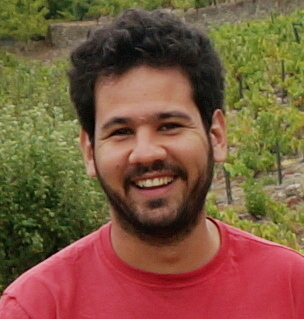
\includegraphics[scale=0.25]{photo.png} %set scale as desired, picture named profile.png
%\end{minipage}

%\center{\textsc{\small{\so{25 y/o, brazilian}}}}

\ifthenelse {\boolean{en}} {\section{Summary}} {\section{Sum�rio}}
\begin{tabularx}{0.96\linewidth}{p{0.96\linewidth}}
	% Acad�mico
\ifthenelse {\boolean{en}} {
    	Ph.D. in Computer Science and Open Source enthusiast working with networks, large-scale data and in how the routinary characteristics of human mobility affect the network traffic demands. Besides, I am passionate about coding, e.g., to design and write APIs, web crawlers, and full-stack web applications. \\
	} {
  		& Doutor em Ci�ncia da Computa��o e entusiasta do Software Livre trabalhando com redes, dados em larga escala e em como a rotina da mobilidade humana afeta as demandas de tr�fego no rede. Al�m disto, eu adoro programar.
}
\end{tabularx}

\ifthenelse {\boolean{en}} {
 	\ifthenelse {\boolean{everything}} {
 		\section{Education}
 		} {
 		\section{Recent Education}
 		}
    } {
		\ifthenelse {\boolean{everything}} {
	 		\section{Educa��o}
	 	} {
	 		\section{Educa��o recente}
	 	}
    }
	\begin{tabularx}{0.97\linewidth}{>{\raggedleft\scshape}p{2.1cm}X}
		\gray \course & \textbf{\cc} \\
		\gray \type & \textbf{\phd} \\
		\gray \period & \textbf{\october 2011 --- \may 2015} \\
		\gray \institution & \textbf{\ecolelinked} {\hfill \france} \\
		& % quebra de linha na gambiarra
	\end{tabularx}

	\begin{tabularx}{0.97\linewidth}{>{\raggedleft\scshape}p{2.1cm}X}
		\gray \course & \textbf{\cc} \\
		\gray \type & \textbf{\master} \\
		\gray \period & \textbf{\march 2009 --- \july 2011} \\
		\gray \institution & \textbf{\ufmglinked} {\hfill \brazil} \\
	    \gray \avgscore & \textbf{94}\% \\
		& % quebra de linha na gambiarra
	\end{tabularx}

	\begin{tabularx}{0.97\linewidth}{>{\raggedleft\scshape}p{2.1cm}X}
		\gray \course & \textbf{\cc} \\
		\gray \type & \textbf{\bachelor} \\
		\gray \period	& \textbf{\august 2004 --- \august 2008} \\
		\gray \institution & \textbf{\puclinked} {\hfill \brazil} \\
	    \gray \avgscore & \textbf{85}\% \\
		& % quebra de linha na gambiarra
	\end{tabularx}

\ifthenelse{\boolean{academy}} {
	% priorizatize academic information
	\ifthenelse {\boolean{en}}{
	\ifthenelse {\boolean{everything}} {
		\section{Academic Experiences}
		} {
		\section{Recent Academic Experiences}
		}
	} {
	\ifthenelse {\boolean{everything}} {
		\section{Experi�ncias Acad�micas}
	} {
		\section{Experi�ncias Acad�micas Recentes}
	}
}

\begin{tabularx}{0.97\linewidth}{>{\raggedleft\scshape}p{2.1cm}X}
	\gray \area & \textbf{\complex, \pand \data} \\
	\gray \project & \textbf{\ifthenelse {\boolean{en}}
							{From Your Routine to Better Network Services}
							{Da Sua Rotina a Melhores Servi�os de Rede}
						  } \\
	\gray \period	& \textbf{\october 2011 --- \december 2014} \\
	\gray \institution & \textbf{\ecole} \\
						   & \ifthenelse {\boolean{en}}
							  {Ph.D Thesis investigated aspects of the human mobility and its impact on the network data traffic, planning and deployment. I've analysed large-scale datasets from mobility and traffic demands generated by millions of users. Several parallelization techniques were used to summarise and assess huge amounts of data. Python multiprocessing, thread and R multicore libraries were largely employed. 5 conference papers were published and 3 journal papers are in submission with the outcomes of this Thesis.}
							  {Minha Tese de Doutorado invesitou v�rios aspectos da mobilidade humana e seu impacto no tr�fego de dados, planejamento e deposi��o. Eu analisei dados em larga escala de mobilidade e demandas de tr�fego geradas por milh�es de usu�rios. Diversas t�cnicas de paralelismo foram empregas para sumarizar e avaliar grandes quantidades de dados. Bibliotecas multiprocessing do Python e multicore do R foram amplamente empregadas neste processo. 5 artigos foram publicados em confer�ncias internacionais e tr�s papers em peri�dicos est�o em submiss�o com o resultados da Tese.} \\
	&
\end{tabularx}

\ifthenelse {\boolean{everything}} {

	\begin{tabularx}{0.97\linewidth}{>{\raggedleft\scshape}p{2.1cm}X}
		\gray \area & \textbf{\wsn, \pand \complex} \\
		\gray \project & \textbf{\ifthenelse {\boolean{en}}
										{Centrality-based Routing for Wireless Sensor Networks}
										{Roteamento Baseado em Centralidade para Redes de Sensores sem Fio}
									} \\
		\gray \period	& \textbf{\march 2009 --- \june 2011} \\
		  \gray \institution & \textbf{\ufmg} \\
								 & \ifthenelse {\boolean{en}}
									{This project aimed to use centrality information on the design of routing algorithms for Wireless Sensor Networks. In this context, two new topological metrics were proposed, distributed algorithms to calculate them, and a tree-based routing algorithms that take advantage of them. Simulators Castalia (C++) and Sinalgo (Java) were used in this project. 1 Conference and 1 Journal paper were published with the results of this Thesis.}
									{Este projeto teve o intuito de usar a informa��o de centralidade no projeto de algoritmos de roteamento para Redes de Sensores sem Fio. Neste contexto, foram propostas duas novas m�tricas de centralidade, algoritmos distribu�dos para o c�lculo das mesmas e algoritmos de roteamento em �rvore baseados nas mesmas. Castalia (C++) e Sinalgo (Java) foram os simuladores empregados neste projeto. Foram publicados 1 paper em confer�ncia e 1 em peri�dico internacional com os resultados desta Disserta��o.} \\
		&
	\end{tabularx}

	\begin{tabularx}{0.97\linewidth}{>{\raggedleft\scshape}p{2.1cm}X}
		\gray \area & \textbf{\wsn} \\
		\gray \project & \textbf{\ifthenelse {\boolean{en}}
									{Data Codification, Fusion and Communication in \wsn}
									{Codifica��o, Fus�o e Comunica��o de Dados em \wsn}
								} \\
		\gray \period	& \textbf{\january 2006 --- \december 2007} \\
		\gray \institution & \textbf{\puc} \\
					 & \ifthenelse {\boolean{en}}
								{This project aimed to create an application for fire detection using a real dataset of weather measurements. A novel way to make data fusion, and codification was proposed. Simulation used NS 2 (C++ and TCL).} 
								{Este projeto teve o intuito de criar uma aplica��o para detec��o de inc�ndios utilizando dados reais de condi��es metereol�gicas. Foram propostos m�todos de fus�o e codifca��o de dados para este cen�rio. Simula��es com Network Simulator 2 (C++ and TCL).} \\
		&
	\end{tabularx}

}{}
		  
%	\begin{tabularx}{0.97\linewidth}{>{\raggedleft\scshape}p{2.1cm}X}
%		\gray \area & \textbf{\wsn} \\
%		\gray \project & \ifthenelse {\boolean{en}}
%                                {\textbf{Game Theory in Decision Making in \wsn}}
%                                {\textbf{Teoria dos Jogos na Tomada de Decis�o em \wsn}}\\
%		\gray \period & \textbf{\january 2007 --- \december 2007} \\
%		\gray \institution & \textbf{\puc} \\
%                    & \ifthenelse {\boolean{en}}
%                                {This project aimed to create an application for fire detection using real data. A novel way to make data fusion, and codification was proposed in this scenario. One simulator was used, Network Simulator (NS-2).} 
%                                {Este projeto teve o intuito de criar uma aplica��o para detec��o de inc�ndios utilizando dados reais. Uma nova maneira de fazer fus�o e codifca��o de dados foi proposta para este cen�rio. Um simulador foi utilizado, Network Simulator (NS-2).} \\
%        &
%	\end{tabularx}

\ifthenelse{\boolean{everything}} {
% Colocar disciplinas relevantes para o foco do curr�culo, only when academic curriculum
	\ifthenelse {\boolean{en}} {\section{Relevant Coursework}} {\section{Disciplinas Relevantes}}
		\begin{tabularx}{0.97\linewidth}{>{\raggedleft\scshape}p{2.1cm}X}
	  		\gray \course & \ifthenelse {\boolean{en}} {\textbf{Design and Analysis of Algorithms}}{\textbf{Projeto e An�lise de Algoritmos}} \\
			\gray \score & \textbf{98\%} \\
			\gray \period & \textbf{\february 2009 --- \july 2009} \\
			\gray \institution & \textbf{\ufmg} \\
		\end{tabularx}

	  \begin{tabularx}{0.97\linewidth}{>{\raggedleft\scshape}p{2.1cm}X}
			\gray \course & \ifthenelse {\boolean{en}} {\textbf{Distributed Algorithms}}{\textbf{Algoritmos Distribu�dos}} \\
			\gray \score & \textbf{100\%} \\
			\gray \period & \textbf{\august 2009 --- \december 2009} \\
			\gray \institution & \textbf{\ufmg} \\
	  \end{tabularx}

	  \begin{tabularx}{0.97\linewidth}{>{\raggedleft\scshape}p{2.1cm}X}
			\gray \course & \ifthenelse {\boolean{en}} {\textbf{Ubiquitous Computing}} {\textbf{Computa��o Ub�qua}} \\
			\gray \score & \textbf{96\%} \\
			\gray \period & \textbf{\august 2008 --- \december 2008} \\
			\gray \institution & \textbf{\ufmg} \\
	  \end{tabularx}

	  \begin{tabularx}{0.97\linewidth}{>{\raggedleft\scshape}p{2.1cm}X}
			\gray \course & \textbf{\complex} \\
			\gray \score & \textbf{90\%} \\
			\gray \period & \textbf{\august 2009 --- \december 2009} \\
		  \gray \institution & \textbf{\ufmg} \\
	  \end{tabularx}

	  \begin{tabularx}{0.97\linewidth}{>{\raggedleft\scshape}p{2.1cm}X}
			\gray \course & \ifthenelse {\boolean{en}} {\textbf{Quantitative Methods and Experimental Design in Computer Science}} {\textbf{M�todos Quantitativos em Ci�ncia da Computa��o Experimental}} \\
			\gray \score & \textbf{92\%} \\
			\gray \period & \textbf{\march 2009 --- \july 2009} \\
			\gray \institution & \textbf{\ufmg} \\
	  \end{tabularx}
}


\ifthenelse {\boolean{en}} {
	\ifthenelse {\boolean{everything}} {
		\section{\href{https://scholar.google.com/citations?user=pD4KMUsAAAAJ}{Publications}}
	}{
		\section{Recent \href{https://scholar.google.com/citations?user=pD4KMUsAAAAJ}{publications}}
	}
} {
	\ifthenelse {\boolean{everything}} {
		\section{\href{https://scholar.google.com/citations?user=pD4KMUsAAAAJ}{Publica��es}}
	} {
		\section{\href{https://scholar.google.com/citations?user=pD4KMUsAAAAJ}{Publica��es} recentes}
	}
}

\begin{tabularx}{0.97\linewidth}{>{\raggedleft\scshape}p{2.1cm}X}
	& Oliveira, Eduardo Mucelli Rezende and Carneiro Viana, Aline and Naveen, K. P. and Sarraute, Carlos., "Analysis and Modeling of Mobile Data Traffic in Mexico City", NetMob, April 2015, Mit Media Lab, Cambridge, MA, United States. \\
	&
\end{tabularx}

\begin{tabularx}{0.97\linewidth}{>{\raggedleft\scshape}p{2.1cm}X}
	& Oliveira, Eduardo Mucelli Rezende and Carneiro Viana, Aline and Naveen, K. P. and Sarraute, Carlos., "Measurement-driven mobile data traffic modeling in a large metropolitan area", IEEE Percom, March 2015, Saint Louis, United States. \\
	&
\end{tabularx}

\begin{tabularx}{0.97\linewidth}{>{\raggedleft\scshape}p{2.1cm}X}
	& Oliveira, Eduardo Mucelli Rezende and Viana, Aline Carneiro., "From Routine to Network Deployment for Data Offloading in Metropolitan Areas", IEEE SECON, June 2014, Singapore. \\
	&
\end{tabularx}

\begin{tabularx}{0.97\linewidth}{>{\raggedleft\scshape}p{2.1cm}X}
	& Oliveira, Eduardo Mucelli Rezende and Viana, Aline Carneiro., "Routine-based Network Deployment", IEEE INFOCOM, Student workshop, April 2014, Toronto, Canada. \\
	&
\end{tabularx}

\ifthenelse {\boolean{everything}} {
	\begin{tabularx}{0.97\linewidth}{>{\raggedleft\scshape}p{2cm}X}
		& Oliveira, Eduardo Mucelli Rezende and Viana, Aline Carneiro., "From Routine To Better Network Services", IEEE/IFIP WMNC, May 2014, Algarve, Portugal. \\
		&
	\end{tabularx}

	\begin{tabularx}{0.97\linewidth}{>{\raggedleft\scshape}p{2cm}X}
		& Oliveira, Eduardo Mucelli Rezende and Viana, Aline Carneiro., "Routine-based network deployment for data offloading in metropolitan areas", IEEE WCNC 2014, Istanbul, Turkey. \\
		&
	\end{tabularx}

	\begin{tabularx}{0.97\linewidth}{>{\raggedleft\scshape}p{2cm}X}
		& Oliveira, Eduardo Mucelli Rezende and Viana, Aline Carneiro., "From your routine to hotspot deployment for data offloading", ACM CoNEXT Student 2012, Nice, France. \\
		&
	\end{tabularx}

	\begin{tabularx}{0.97\linewidth}{>{\raggedleft\scshape}p{2cm}X}
		& Oliveira, Eduardo M. R., Ramos, Heitor S., Loureiro, Antonio A. F., "Centrality-based routing for Wireless Sensor Networks", IEEE Wireless Days (WD), 2010 IFIP, Venice, Italy. \\
		&
	\end{tabularx}

	\begin{tabularx}{0.97\linewidth}{>{\raggedleft\scshape}p{2cm}X}
		& Oliveira, Eduardo Mucelli Rezende, O. S. V. M., Pedro, Mini, R. A. F.
		Comunica��o, Codifica��o e Fus�o de Dados para uma Aplica��o de Detec��o de Inc�ndios utilizando Redes de Sensores sem Fio \textit{("Data Codification, Fusion and Communication in Wireless Sensors Networks")}, 1� Workshop on Pervasive and Ubiquitous Computing, 2007, Gramado, RS, Brazil.
	% & % descomentar quando adicionar um campo abaixo -- adicionar o \\ na linha anterior
	\end{tabularx}
}{}
	\section{Professional Experiences}
\newcommand*{\cvsimple}[4][.25em]{
\begin{tabular*}{\maincolumnwidth}{l@{\extracolsep{\fill}}r}%
	% {\bfseries #4} & {\bfseries #5}\\%
	{\itshape #3} & {\itshape #2}\\%
\end{tabular*}%
\ifx&#4&%
\else{\\%
	\begin{minipage}{\maincolumnwidth}%
		\small#4%
\end{minipage}}\fi%
\par\addvspace{#1}}

\cventry{\january 2023 -- Present}{\sse}{Synthesia}{Remote}{}{
	Working on improving the robustness of the video generation.
}
\cventry{\december 2021 -- \november 2022}{\seii}{Canonical}{Remote}{}{
	Improving the data pipeline Python codebase to serve technical and non-technical internal teams.
	Working on the service behind \href{https://ubuntu.com/security/livepatch}{Livepatch} in Golang.
}
% Add second entry to the same company https://tex.stackexchange.com/a/294612
\cvsimple{\june 2020 -- \november 2021}{\se}{
	Working on the services behind \href{https://ubuntu.com/advantage}{Ubuntu Advantage} in Golang and Python.
	Introduced a BDD suite to our main Golang services.
	Revamping team's data pipelines: large refactoring of the Python codebase, type checking, linting, moving from Openstack to Kubernetes (Argo), Grafana, Prometheus, Pushgateway, alerting.
}
\cventry{\july 2016 -- \may 2020}{\se}{BlaBlaCar}{\protect\france}{}{
	Developed features, optimized performance, deployed and monitored a dozen of Java services at the Trip Search team. \href{https://medium.com/blablacar-tech/fast-machine-learning-predictions-6856b3623e5}{Wrote and integrated the first library} to handle Machine Learning predictions at scale for \href{https://github.com/edumucelli/benchmark-xgboost-java}{which I have extensively measured performance}. Significantly worked on the \href{https://blog.blablacar.com/newsroom/news-list/new-search-logo-visual-identity}{new search, routing and matching algorithm}. Main technologies were Java, Elasticsearch, PostgreSQL, PostGIS, XGBoost, OSRM, MySQL and Redis, R and Python.
}
\cventry{\june 2015 -- \june 2016}{Postdoctoral Researcher}{Orange}{\protect\france}{}{
	Developed machine-learning assisted techniques to predict users' QoE based on network's KPIs.
}
\cventry{\july 2011 --- \september 2011}{\se}{Dito Internet}{\protect\brazil}{}{
	Developed in Ruby on Rails, as part of a team, Telecom Italia Mobile's project called TIM Beta, \textit{\href{www.timbeta.com.br}{timbeta.com.br}}.
}
\cventry{\november 2010 --- \may 2011}{Researcher Intern}{Telecom Italia Future Centre}{\protect\italy}{}{
	Developed, in Python, a project called Future of Enterprises aiming to improve the real-time interaction among employees.
}
\cventry{\february 2008 --- \february 2009}{\se}{Task Internet}{\protect\brazil}{}{
	Lead developer of a social network in Ruby on Rails.
}
}{
	% priorizatize professional information
	\section{Professional Experiences}
\newcommand*{\cvsimple}[4][.25em]{
\begin{tabular*}{\maincolumnwidth}{l@{\extracolsep{\fill}}r}%
	% {\bfseries #4} & {\bfseries #5}\\%
	{\itshape #3} & {\itshape #2}\\%
\end{tabular*}%
\ifx&#4&%
\else{\\%
	\begin{minipage}{\maincolumnwidth}%
		\small#4%
\end{minipage}}\fi%
\par\addvspace{#1}}

\cventry{\january 2023 -- Present}{\sse}{Synthesia}{Remote}{}{
	Working on improving the robustness of the video generation.
}
\cventry{\december 2021 -- \november 2022}{\seii}{Canonical}{Remote}{}{
	Improving the data pipeline Python codebase to serve technical and non-technical internal teams.
	Working on the service behind \href{https://ubuntu.com/security/livepatch}{Livepatch} in Golang.
}
% Add second entry to the same company https://tex.stackexchange.com/a/294612
\cvsimple{\june 2020 -- \november 2021}{\se}{
	Working on the services behind \href{https://ubuntu.com/advantage}{Ubuntu Advantage} in Golang and Python.
	Introduced a BDD suite to our main Golang services.
	Revamping team's data pipelines: large refactoring of the Python codebase, type checking, linting, moving from Openstack to Kubernetes (Argo), Grafana, Prometheus, Pushgateway, alerting.
}
\cventry{\july 2016 -- \may 2020}{\se}{BlaBlaCar}{\protect\france}{}{
	Developed features, optimized performance, deployed and monitored a dozen of Java services at the Trip Search team. \href{https://medium.com/blablacar-tech/fast-machine-learning-predictions-6856b3623e5}{Wrote and integrated the first library} to handle Machine Learning predictions at scale for \href{https://github.com/edumucelli/benchmark-xgboost-java}{which I have extensively measured performance}. Significantly worked on the \href{https://blog.blablacar.com/newsroom/news-list/new-search-logo-visual-identity}{new search, routing and matching algorithm}. Main technologies were Java, Elasticsearch, PostgreSQL, PostGIS, XGBoost, OSRM, MySQL and Redis, R and Python.
}
\cventry{\june 2015 -- \june 2016}{Postdoctoral Researcher}{Orange}{\protect\france}{}{
	Developed machine-learning assisted techniques to predict users' QoE based on network's KPIs.
}
\cventry{\july 2011 --- \september 2011}{\se}{Dito Internet}{\protect\brazil}{}{
	Developed in Ruby on Rails, as part of a team, Telecom Italia Mobile's project called TIM Beta, \textit{\href{www.timbeta.com.br}{timbeta.com.br}}.
}
\cventry{\november 2010 --- \may 2011}{Researcher Intern}{Telecom Italia Future Centre}{\protect\italy}{}{
	Developed, in Python, a project called Future of Enterprises aiming to improve the real-time interaction among employees.
}
\cventry{\february 2008 --- \february 2009}{\se}{Task Internet}{\protect\brazil}{}{
	Lead developer of a social network in Ruby on Rails.
}
	\ifthenelse {\boolean{en}}{
	\ifthenelse {\boolean{everything}} {
		\section{Academic Experiences}
		} {
		\section{Recent Academic Experiences}
		}
	} {
	\ifthenelse {\boolean{everything}} {
		\section{Experi�ncias Acad�micas}
	} {
		\section{Experi�ncias Acad�micas Recentes}
	}
}

\begin{tabularx}{0.97\linewidth}{>{\raggedleft\scshape}p{2.1cm}X}
	\gray \area & \textbf{\complex, \pand \data} \\
	\gray \project & \textbf{\ifthenelse {\boolean{en}}
							{From Your Routine to Better Network Services}
							{Da Sua Rotina a Melhores Servi�os de Rede}
						  } \\
	\gray \period	& \textbf{\october 2011 --- \december 2014} \\
	\gray \institution & \textbf{\ecole} \\
						   & \ifthenelse {\boolean{en}}
							  {Ph.D Thesis investigated aspects of the human mobility and its impact on the network data traffic, planning and deployment. I've analysed large-scale datasets from mobility and traffic demands generated by millions of users. Several parallelization techniques were used to summarise and assess huge amounts of data. Python multiprocessing, thread and R multicore libraries were largely employed. 5 conference papers were published and 3 journal papers are in submission with the outcomes of this Thesis.}
							  {Minha Tese de Doutorado invesitou v�rios aspectos da mobilidade humana e seu impacto no tr�fego de dados, planejamento e deposi��o. Eu analisei dados em larga escala de mobilidade e demandas de tr�fego geradas por milh�es de usu�rios. Diversas t�cnicas de paralelismo foram empregas para sumarizar e avaliar grandes quantidades de dados. Bibliotecas multiprocessing do Python e multicore do R foram amplamente empregadas neste processo. 5 artigos foram publicados em confer�ncias internacionais e tr�s papers em peri�dicos est�o em submiss�o com o resultados da Tese.} \\
	&
\end{tabularx}

\ifthenelse {\boolean{everything}} {

	\begin{tabularx}{0.97\linewidth}{>{\raggedleft\scshape}p{2.1cm}X}
		\gray \area & \textbf{\wsn, \pand \complex} \\
		\gray \project & \textbf{\ifthenelse {\boolean{en}}
										{Centrality-based Routing for Wireless Sensor Networks}
										{Roteamento Baseado em Centralidade para Redes de Sensores sem Fio}
									} \\
		\gray \period	& \textbf{\march 2009 --- \june 2011} \\
		  \gray \institution & \textbf{\ufmg} \\
								 & \ifthenelse {\boolean{en}}
									{This project aimed to use centrality information on the design of routing algorithms for Wireless Sensor Networks. In this context, two new topological metrics were proposed, distributed algorithms to calculate them, and a tree-based routing algorithms that take advantage of them. Simulators Castalia (C++) and Sinalgo (Java) were used in this project. 1 Conference and 1 Journal paper were published with the results of this Thesis.}
									{Este projeto teve o intuito de usar a informa��o de centralidade no projeto de algoritmos de roteamento para Redes de Sensores sem Fio. Neste contexto, foram propostas duas novas m�tricas de centralidade, algoritmos distribu�dos para o c�lculo das mesmas e algoritmos de roteamento em �rvore baseados nas mesmas. Castalia (C++) e Sinalgo (Java) foram os simuladores empregados neste projeto. Foram publicados 1 paper em confer�ncia e 1 em peri�dico internacional com os resultados desta Disserta��o.} \\
		&
	\end{tabularx}

	\begin{tabularx}{0.97\linewidth}{>{\raggedleft\scshape}p{2.1cm}X}
		\gray \area & \textbf{\wsn} \\
		\gray \project & \textbf{\ifthenelse {\boolean{en}}
									{Data Codification, Fusion and Communication in \wsn}
									{Codifica��o, Fus�o e Comunica��o de Dados em \wsn}
								} \\
		\gray \period	& \textbf{\january 2006 --- \december 2007} \\
		\gray \institution & \textbf{\puc} \\
					 & \ifthenelse {\boolean{en}}
								{This project aimed to create an application for fire detection using a real dataset of weather measurements. A novel way to make data fusion, and codification was proposed. Simulation used NS 2 (C++ and TCL).} 
								{Este projeto teve o intuito de criar uma aplica��o para detec��o de inc�ndios utilizando dados reais de condi��es metereol�gicas. Foram propostos m�todos de fus�o e codifca��o de dados para este cen�rio. Simula��es com Network Simulator 2 (C++ and TCL).} \\
		&
	\end{tabularx}

}{}
		  
%	\begin{tabularx}{0.97\linewidth}{>{\raggedleft\scshape}p{2.1cm}X}
%		\gray \area & \textbf{\wsn} \\
%		\gray \project & \ifthenelse {\boolean{en}}
%                                {\textbf{Game Theory in Decision Making in \wsn}}
%                                {\textbf{Teoria dos Jogos na Tomada de Decis�o em \wsn}}\\
%		\gray \period & \textbf{\january 2007 --- \december 2007} \\
%		\gray \institution & \textbf{\puc} \\
%                    & \ifthenelse {\boolean{en}}
%                                {This project aimed to create an application for fire detection using real data. A novel way to make data fusion, and codification was proposed in this scenario. One simulator was used, Network Simulator (NS-2).} 
%                                {Este projeto teve o intuito de criar uma aplica��o para detec��o de inc�ndios utilizando dados reais. Uma nova maneira de fazer fus�o e codifca��o de dados foi proposta para este cen�rio. Um simulador foi utilizado, Network Simulator (NS-2).} \\
%        &
%	\end{tabularx}

\ifthenelse{\boolean{everything}} {
% Colocar disciplinas relevantes para o foco do curr�culo, only when academic curriculum
	\ifthenelse {\boolean{en}} {\section{Relevant Coursework}} {\section{Disciplinas Relevantes}}
		\begin{tabularx}{0.97\linewidth}{>{\raggedleft\scshape}p{2.1cm}X}
	  		\gray \course & \ifthenelse {\boolean{en}} {\textbf{Design and Analysis of Algorithms}}{\textbf{Projeto e An�lise de Algoritmos}} \\
			\gray \score & \textbf{98\%} \\
			\gray \period & \textbf{\february 2009 --- \july 2009} \\
			\gray \institution & \textbf{\ufmg} \\
		\end{tabularx}

	  \begin{tabularx}{0.97\linewidth}{>{\raggedleft\scshape}p{2.1cm}X}
			\gray \course & \ifthenelse {\boolean{en}} {\textbf{Distributed Algorithms}}{\textbf{Algoritmos Distribu�dos}} \\
			\gray \score & \textbf{100\%} \\
			\gray \period & \textbf{\august 2009 --- \december 2009} \\
			\gray \institution & \textbf{\ufmg} \\
	  \end{tabularx}

	  \begin{tabularx}{0.97\linewidth}{>{\raggedleft\scshape}p{2.1cm}X}
			\gray \course & \ifthenelse {\boolean{en}} {\textbf{Ubiquitous Computing}} {\textbf{Computa��o Ub�qua}} \\
			\gray \score & \textbf{96\%} \\
			\gray \period & \textbf{\august 2008 --- \december 2008} \\
			\gray \institution & \textbf{\ufmg} \\
	  \end{tabularx}

	  \begin{tabularx}{0.97\linewidth}{>{\raggedleft\scshape}p{2.1cm}X}
			\gray \course & \textbf{\complex} \\
			\gray \score & \textbf{90\%} \\
			\gray \period & \textbf{\august 2009 --- \december 2009} \\
		  \gray \institution & \textbf{\ufmg} \\
	  \end{tabularx}

	  \begin{tabularx}{0.97\linewidth}{>{\raggedleft\scshape}p{2.1cm}X}
			\gray \course & \ifthenelse {\boolean{en}} {\textbf{Quantitative Methods and Experimental Design in Computer Science}} {\textbf{M�todos Quantitativos em Ci�ncia da Computa��o Experimental}} \\
			\gray \score & \textbf{92\%} \\
			\gray \period & \textbf{\march 2009 --- \july 2009} \\
			\gray \institution & \textbf{\ufmg} \\
	  \end{tabularx}
}


\ifthenelse {\boolean{en}} {
	\ifthenelse {\boolean{everything}} {
		\section{\href{https://scholar.google.com/citations?user=pD4KMUsAAAAJ}{Publications}}
	}{
		\section{Recent \href{https://scholar.google.com/citations?user=pD4KMUsAAAAJ}{publications}}
	}
} {
	\ifthenelse {\boolean{everything}} {
		\section{\href{https://scholar.google.com/citations?user=pD4KMUsAAAAJ}{Publica��es}}
	} {
		\section{\href{https://scholar.google.com/citations?user=pD4KMUsAAAAJ}{Publica��es} recentes}
	}
}

\begin{tabularx}{0.97\linewidth}{>{\raggedleft\scshape}p{2.1cm}X}
	& Oliveira, Eduardo Mucelli Rezende and Carneiro Viana, Aline and Naveen, K. P. and Sarraute, Carlos., "Analysis and Modeling of Mobile Data Traffic in Mexico City", NetMob, April 2015, Mit Media Lab, Cambridge, MA, United States. \\
	&
\end{tabularx}

\begin{tabularx}{0.97\linewidth}{>{\raggedleft\scshape}p{2.1cm}X}
	& Oliveira, Eduardo Mucelli Rezende and Carneiro Viana, Aline and Naveen, K. P. and Sarraute, Carlos., "Measurement-driven mobile data traffic modeling in a large metropolitan area", IEEE Percom, March 2015, Saint Louis, United States. \\
	&
\end{tabularx}

\begin{tabularx}{0.97\linewidth}{>{\raggedleft\scshape}p{2.1cm}X}
	& Oliveira, Eduardo Mucelli Rezende and Viana, Aline Carneiro., "From Routine to Network Deployment for Data Offloading in Metropolitan Areas", IEEE SECON, June 2014, Singapore. \\
	&
\end{tabularx}

\begin{tabularx}{0.97\linewidth}{>{\raggedleft\scshape}p{2.1cm}X}
	& Oliveira, Eduardo Mucelli Rezende and Viana, Aline Carneiro., "Routine-based Network Deployment", IEEE INFOCOM, Student workshop, April 2014, Toronto, Canada. \\
	&
\end{tabularx}

\ifthenelse {\boolean{everything}} {
	\begin{tabularx}{0.97\linewidth}{>{\raggedleft\scshape}p{2cm}X}
		& Oliveira, Eduardo Mucelli Rezende and Viana, Aline Carneiro., "From Routine To Better Network Services", IEEE/IFIP WMNC, May 2014, Algarve, Portugal. \\
		&
	\end{tabularx}

	\begin{tabularx}{0.97\linewidth}{>{\raggedleft\scshape}p{2cm}X}
		& Oliveira, Eduardo Mucelli Rezende and Viana, Aline Carneiro., "Routine-based network deployment for data offloading in metropolitan areas", IEEE WCNC 2014, Istanbul, Turkey. \\
		&
	\end{tabularx}

	\begin{tabularx}{0.97\linewidth}{>{\raggedleft\scshape}p{2cm}X}
		& Oliveira, Eduardo Mucelli Rezende and Viana, Aline Carneiro., "From your routine to hotspot deployment for data offloading", ACM CoNEXT Student 2012, Nice, France. \\
		&
	\end{tabularx}

	\begin{tabularx}{0.97\linewidth}{>{\raggedleft\scshape}p{2cm}X}
		& Oliveira, Eduardo M. R., Ramos, Heitor S., Loureiro, Antonio A. F., "Centrality-based routing for Wireless Sensor Networks", IEEE Wireless Days (WD), 2010 IFIP, Venice, Italy. \\
		&
	\end{tabularx}

	\begin{tabularx}{0.97\linewidth}{>{\raggedleft\scshape}p{2cm}X}
		& Oliveira, Eduardo Mucelli Rezende, O. S. V. M., Pedro, Mini, R. A. F.
		Comunica��o, Codifica��o e Fus�o de Dados para uma Aplica��o de Detec��o de Inc�ndios utilizando Redes de Sensores sem Fio \textit{("Data Codification, Fusion and Communication in Wireless Sensors Networks")}, 1� Workshop on Pervasive and Ubiquitous Computing, 2007, Gramado, RS, Brazil.
	% & % descomentar quando adicionar um campo abaixo -- adicionar o \\ na linha anterior
	\end{tabularx}
}{}
}
\ifthenelse{\boolean{en}} {\section{Awards}\label{sec:awards}}
                          {\section{Prêmios}\label{sec:awards}}
	
	\begin{tabularx}{0.97\linewidth}{>{\raggedleft\scshape}p{2.1cm}X}
		\gray \ptitle & \textbf{\ifthenelse{\boolean{en}}{Honorary mention}{Menção honrosa}} \\
		\gray \issuer & \textbf{\ifthenelse{\boolean{en}}{Brazilian Ministry of Justice}{Ministério da Justiça}} \\
		\gray \ifthenelse{\boolean{en}}{Date}{Data} & \textbf{\may 2013} \\
		      & \ifthenelse{\boolean{en}}
		        {Open Data Applications Contest. Lead developer of a Ruby on Rails application called Proconfie. Refer to the Section \hyperref[sec:web_app]{Web Applications} for more details about \hyperref[proconfie]{Proconfie}.}
		        {1\textsuperscript{o} Concurso de Aplicativos do Ministério da Justiça. Desenvolvedor do aplicativo Proconfie. Veja a seção \hyperref[sec:web_app]{Aplicativos Web} para mais detalhes sobre o \hyperref[proconfie]{Proconfie}.} \\
		&
	\end{tabularx}
	
	\begin{tabularx}{0.97\linewidth}{>{\raggedleft\scshape}p{2.1cm}X}
		\gray \ptitle & \textbf{\ifthenelse{\boolean{en}}{Silver Medal}{Medalha de Prata}} \\
		\gray \issuer & \textbf{\puc} \\
		\gray \ifthenelse{\boolean{en}}{Date}{Data} & \textbf{\july 2008} \\
		      & \ifthenelse{\boolean{en}}
		        {Second best overall score during the bachelor.}
		        {Segunda melhor nota total durante todo a graduação.} \\
		&
	\end{tabularx}
	
	\begin{tabularx}{0.97\linewidth}{>{\raggedleft\scshape}p{2.1cm}X}
		\gray \ptitle & \textbf{\ifthenelse{\boolean{en}}{Honorary mention}{Menção honrosa}} \\
		\gray \issuer & \textbf{\puc} \\
		\gray \ifthenelse{\boolean{en}}{Date}{Data} & \textbf{\may 2007} \\
		      & \ifthenelse{\boolean{en}}
		        {For the work "Game Theory in Decision Making in Wireless Sensor Networks" presented in the 15\textsuperscript{th} Sciences Seminar.}
				{Para o trabalho "Teoria dos Jogos na Tomada de Decisão em Redes de Sensores Sem Fio" apresentado no 15\textsuperscript{o} Seminário de Ciências Exatas.} \\
		&
	\end{tabularx}

% Not adding it for now, if requested for an interview, add this part back and print the curriculum
% \ifthenelse{\boolean{en}}{\section{Personal References}}{\section{Refer�ncias Pessoais}}
	\begin{tabularx}{\linewidth}{>{\raggedleft\scshape}p{2.1cm}X}
    \ifthenelse{\boolean{en}}{
		& Aline Carneiro Viana. Research Scientist, INRIA, France. \linebreak {\carta} aline.viana@inria.fr \\
		& \\
		& Antonio A. F. Loureiro. Titular Professor of the Computer Science Department at Federal University of Minas Gerais, Brazil. {\carta}~loureiro@dcc.ufmg.br \\
		& \\
		& Pedro Olmo S. V. de Melo. Professor of the Computer Science Department at Federal University of Minas Gerais, Brazil. {\carta}~olmo@dcc.ufmg.br \\
		& \\
		& Heitor S. Ramos. Professor of the Institute of Computing at Federal University of Alagoas, Brazil. {\carta}~ramosh@acm.org \\
		& \\
		& Leandro A. Villas. Professor of the Computing Systems Department at State University of Campinas, Brazil. {\carta}~leandro@ic.unicamp.br \\
		& \\
		& Carlos Sarraute, Director of R\&D at GranData, Argentina. {\carta}~charles@grandata.com \\
		& \\
		& Raquel A. F. Mini. Coordinator of Computer Science Department in Pontifical Catholic University of Minas Gerais, Brazil. {\carta}~raquelmini@pucminas.br\\
		& \\
		& Tales Lacerda. Director of Task Software, Minas Gerais, Belo Horizonte, Brazil. {\carta}~tales@task.com.br \\
    } {
    & Aline Carneiro Viana. Cientista Pesquisadora, INRIA, Fran�a. {\carta}~aline.viana@inria.fr \\
		& \\
    & Antonio A. F. Loureiro. Professor Titular do Departamento de \cc da \ufmg. {\carta}~loureiro@dcc.ufmg.br \\
		& \\
		& Pedro Olmo Stancioli Vaz de Melo. Professor do Departamento de \cc da \ufmg. {\carta}~olmo@dcc.ufmg.br \\
		& \\
		& Heitor S. Ramos. Professor do Instituto de Computa��o na Universidade Federal de Alagoas. {\carta}~ramosh@acm.org \\
		& \\
		& Leandro Aparecido Villas. Professor do Departamento de Sistemas de Computa��o na Unicamp. {\carta}~leandro@ic.unicamp.br \\
		& \\
		& Carlos Sarraute, Diretor de R\&D na GranData, Argentina. {\carta}~charles@grandata.com \\
		& \\
		& Raquel A. F. Mini. Coordenadora do Curso de Ci�ncia da Computa��o na \puc. {\carta}~raquelmini@pucminas.br\\
		& \\
		& Tales Lacerda. Diretor da Task Software, Belo Horizonte, Minas Gerais. {\carta}~tales@task.com.br \\
    }
	\end{tabularx}

\end{center}
\end{document}